\chapter{Implementación y pruebas}\label{cap:implementacion_y_pruebas}

Una vez establecida la base arquitectónica y el diseño del sistema, corresponde abordar la materialización técnica de la plataforma, transformando los requisitos y decisiones de diseño arquitectónico previamente definidos en componentes funcionales de software. Para ello, en primer lugar se detallan los módulos críticos de la implementación tanto en el \textit{backend} como en el \textit{frontend}, haciendo especial énfasis en la sincronización en tiempo real y la seguridad. Posteriormente, se expone la estrategia integral de pruebas, los criterios de calidad adoptados y los resultados de cobertura obtenidos para garantizar la robustez del sistema.

\section{Componentes clave e implementación del sistema}\label{sec:componentes_clave}

En esta sección se exponen los aspectos más representativos del núcleo de \textit{Quizzie}, analizando las decisiones de diseño y patrones de software adoptados para dar respuesta a los requisitos funcionales más complejos: la comunicación bidireccional, la gestión del ciclo de vida de las salas y la seguridad del estado en el \textit{frontend}.

\subsection{Comunicación en tiempo real mediante WebSockets}\label{subsec:impl_websockets}

La interactividad en vivo entre el profesor y los alumnos requiere una arquitectura de baja latencia capaz de difundir eventos de forma simultánea a múltiples clientes mediante el protocolo WebSocket~\cite{websocket_protocol}.

\subsubsection{Gestor de conexiones en el backend (\texttt{ConnectionManager})}
En la ruta \texttt{backend/routers/stage.py}, el gestor de conexiones implementa una adaptación concurrente del patrón de diseño \textit{Observer}~\cite{gamma1994design} combinada con una arquitectura de publicación-suscripción (\textit{Pub-Sub})~\cite{eugster2003pubsub}, permitiendo registrar, desacoplar y administrar dinámicamente el ciclo de vida de las instancias activas de \texttt{WebSocket} asociadas a cada sala mediante su identificador único (\texttt{room\_id}).

\begin{figure}[H]
  \centering
  \makebox[\textwidth][c]{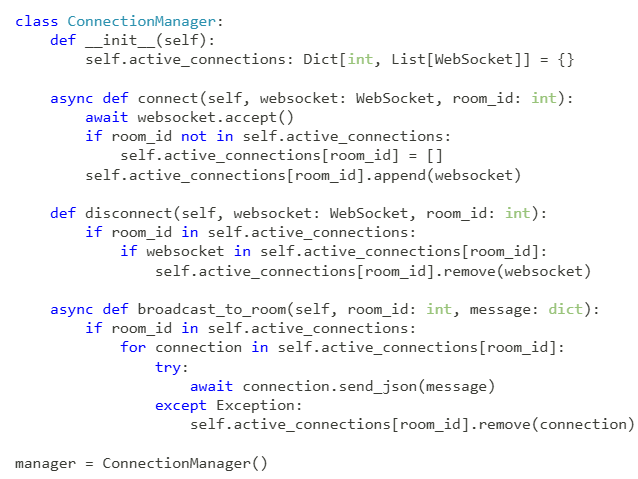
\includegraphics[width=0.9\textwidth]{listings/gestor_conexiones_backend.png}}
  \captionof{lstlisting}{Gestor de conexiones en el \textit{backend}}
  \label{lst:gestor_conexiones_backend}
\end{figure}

Esta estructura permite emitir mensajes masivos con formato JSON mediante el método \texttt{broadcast\_to\_room}. Asimismo, incluye un mecanismo de tolerancia a fallos en bloque \texttt{try-except} que elimina automáticamente las conexiones diferidas o corruptas sin interrumpir la emisión hacia el resto de los participantes.

\newpage

\subsubsection{Suscripción y recepción de eventos en el cliente React}
En el \textit{frontend}, el componente establece la conexión WebSocket con el servidor enviando el parámetro del rol (\texttt{teacher} o \texttt{student}) como parámetro de consulta.

\begin{figure}[H]
  \centering
  \makebox[\textwidth][c]{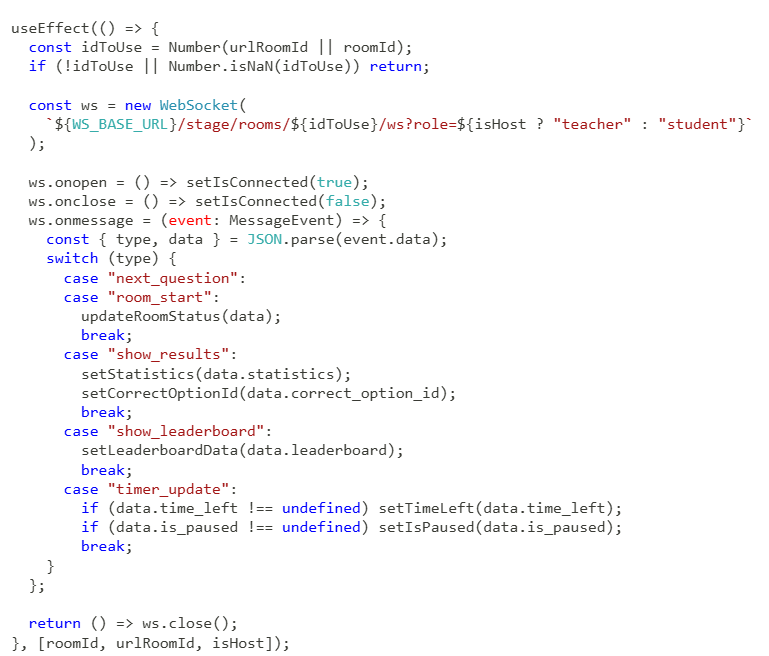
\includegraphics[width=1.1\textwidth]{listings/recepcion_eventos_react.png}}
  \captionof{lstlisting}{Conexión y enrutamiento de eventos WebSocket en React}
  \label{lst:recepcion_eventos_react}
\end{figure}

El \textit{handler} \texttt{onmessage} actúa como un enrutador de eventos de la interfaz de usuario, mutando el estado local de React en función del tipo de evento recibido. Asimismo, la función de retorno del \textit{hook} \texttt{useEffect} (\textit{cleanup function}) garantiza el cierre formal del socket al desmontar el componente, previniendo fugas de memoria.

\newpage

\subsection{Gestión de sala, estado, tiempo y aleatoriedad}\label{subsec:impl_state_time}

El correcto funcionamiento de las sesiones depende de mantener la sala sincronizada y lista para todos los usuarios. Para lograrlo, el servidor asume el control centralizado de los eventos y las decisiones críticas, gestionando el avance del estado de la sala y evitando depender del estado o el reloj individual de cada cliente.

\subsubsection{Cálculo determinista del tiempo restante en UTC}
En \texttt{backend/routers/stage.py}, la medición del tiempo no depende del reloj del cliente, sino de la diferencia estricta de marcas temporales en UTC.

\begin{figure}[H]
  \centering
  \makebox[\textwidth][c]{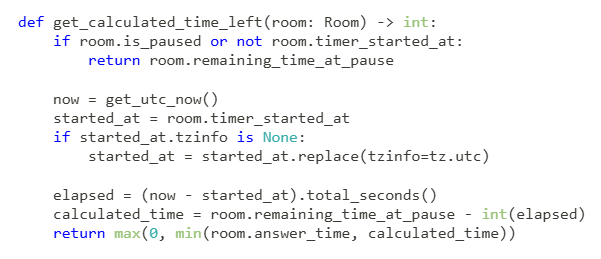
\includegraphics[width=0.9\textwidth]{listings/calculo_tiempo_utc.png}}
  \captionof{lstlisting}{Cálculo determinista del tiempo restante en el servidor}
  \label{lst:calculo_tiempo_utc}
\end{figure}

Al restar el instante actual (\texttt{get\_utc\_now()}) del momento de inicio (\texttt{timer\_started\_at}), el sistema inmuniza la cuenta atrás frente a retrasos de red o pausas de ejecución en el cliente.

\newpage

\subsubsection{Pausa automática por desconexión del profesor}
Para mitigar imprevistos técnicos durante una sesión presencial, el servidor detecta si la conexión WebSocket del docente cae inesperadamente.

\begin{figure}[H]
  \centering
  \makebox[\textwidth][c]{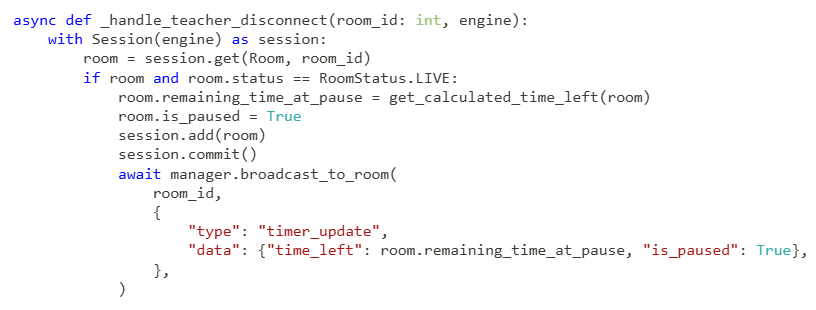
\includegraphics[width=1.1\textwidth]{listings/desconexion_profesor.png}}
  \captionof{lstlisting}{Gestión de desconexión imprevista del profesor}
  \label{lst:desconexion_profesor}
\end{figure}

La función congela la partida almacenando el tiempo restante exacto en \texttt{remaining\_time\_at\_pause} mediante \texttt{get\_calculated\_time\_left} y notifica inmediatamente a todos los estudiantes, pausando la interfaz hasta la reconexión del profesor.

\subsubsection{Barajado determinista de opciones}
Para evitar que los estudiantes copien observando la opción seleccionada en la pantalla de un compañero, el \textit{backend} desordena las opciones mediante una semilla \textit{hash}.

\begin{figure}[H]
  \centering
  \makebox[\textwidth][c]{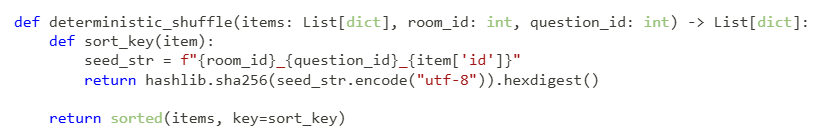
\includegraphics[width=1.1\textwidth]{listings/barajado_anticopia.png}}
  \captionof{lstlisting}{Algoritmo de barajado determinista anti-copia}
  \label{lst:barajado_anticopia}
\end{figure}

El algoritmo genera un \textit{hash SHA-256} combinando la sala, la pregunta y la opción. Esto altera la disposición de las respuestas para cada partida pero mantiene un orden idéntico si un alumno reconecta o recarga su cliente.

\subsubsection{Transición de preguntas y fase de verificación}
El endpoint \texttt{PATCH /rooms/:room\_id/next-question} coordina el avance del cuestionario o la transición a la fase final.

\begin{figure}[H]
  \centering
  \makebox[\textwidth][c]{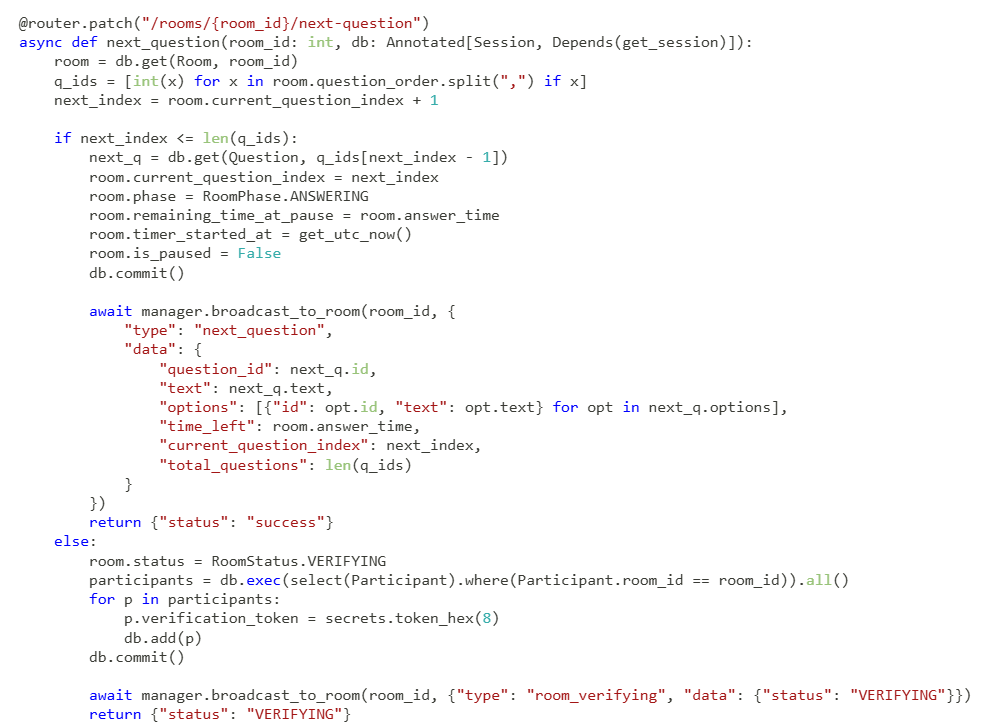
\includegraphics[width=1.2\textwidth]{listings/siguiente_pregunta_verificacion.png}}
  \captionof{lstlisting}{Avance de pregunta y paso a siguiente fase}
  \label{lst:siguiente_pregunta_verificacion}
\end{figure}

Si restan preguntas por responder, el controlador actualiza el índice y emite el evento correspondiente. Al agotar la batería de preguntas, la sala cambia al estado \texttt{VERIFYING} y genera tokens criptográficos efímeros mediante \texttt{secrets.token\_hex(8)}.

\newpage

\subsubsection{Verificación presencial mediante código QR}
Una vez concluida la partida, el resultado acumulado debe ser validado por el docente escaneando un código QR en el dispositivo del alumno.

\begin{figure}[H]
  \centering
  \makebox[\textwidth][c]{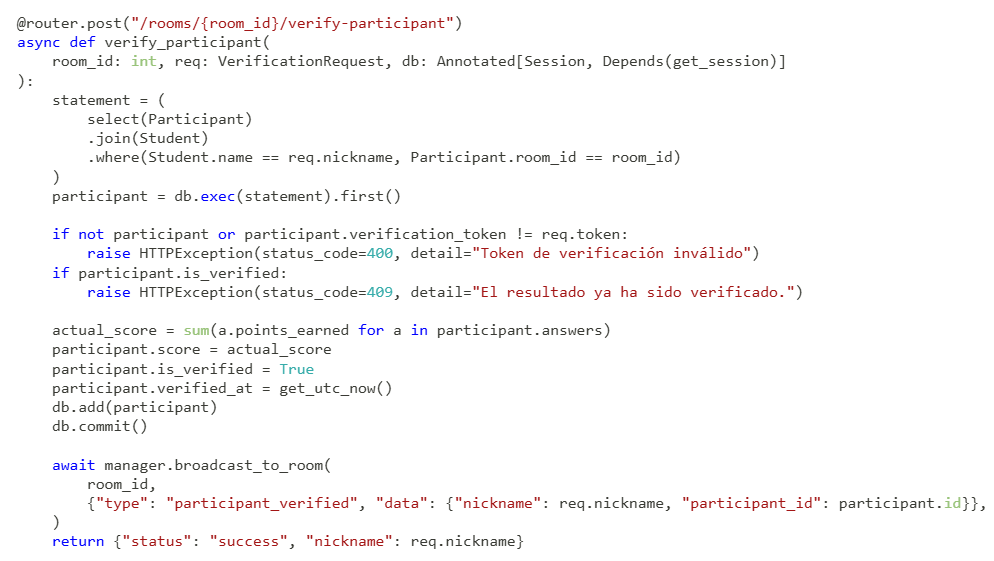
\includegraphics[width=1.2\textwidth]{listings/verificacion_presencial_qr.png}}
  \captionof{lstlisting}{Validación presencial del participante mediante token QR}
  \label{lst:verificacion_presencial_qr}
\end{figure}

El controlador valida el token efímero (\texttt{req.token}), recalcula la puntuación final sumando los puntos auditados, marca al participante como verificado y notifica la confirmación en tiempo real.

\newpage

\subsection{Seguridad, contexto y autenticación}\label{subsec:impl_security_context}

Este bloque aborda el tratamiento del estado del jugador, el saneamiento de datos en la SPA y la protección de endpoints sensibles mediante tokens JWT.

\subsubsection{Persistencia y saneamiento de estado en la SPA}
En \texttt{RoomContext} se encapsula la gestión de la sesión del jugador mediante la \textit{API Context} de React.

\begin{figure}[H]
  \centering
  \makebox[\textwidth][c]{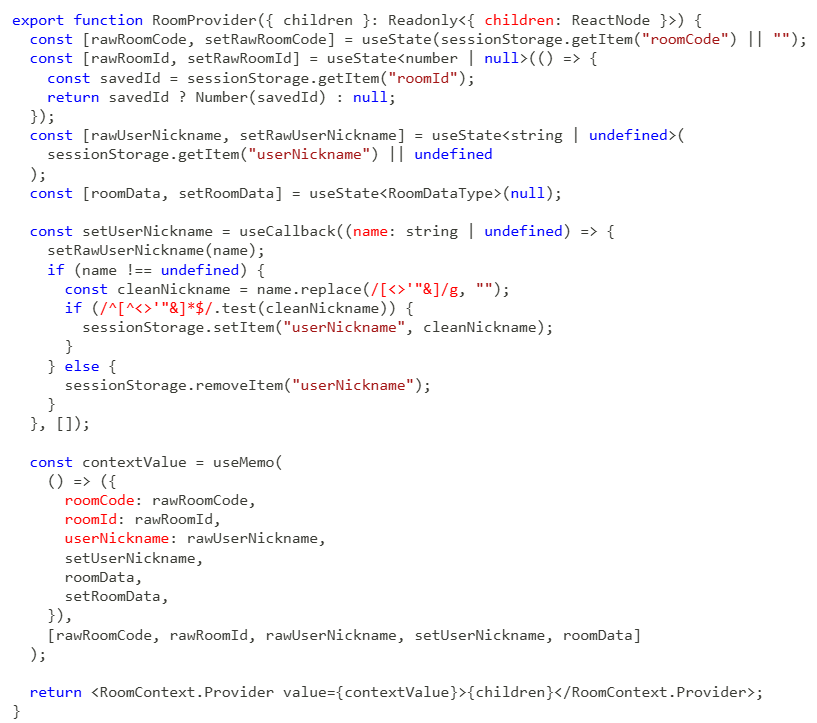
\includegraphics[width=1.05\textwidth]{listings/contexto_sala.png}}
  \captionof{lstlisting}{Gestión del contexto de la sala}
  \label{lst:contexto_sala}
\end{figure}

El componente recupera de forma síncrona los identificadores desde \texttt{sessionStorage} para garantizar la persistencia del estado frente a recargas accidentales del navegador. Asimismo, se aplica una función de saneamiento que purga caracteres sensibles (\texttt{<, >, ', ", \&}) antes de su persistencia y renderizado, mitigando vectores de ataque por inyección de scripts en sitios cruzados o XSS (\textit{Cross-Site Scripting}) \cite{owaspTop10, zalewski2011tangold}.

\subsubsection{Autenticación y protección de endpoints con JWT}
En \texttt{backend/auth.py}, se implementa un mecanismo de inyección de dependencias para autenticar las peticiones de los docentes mediante cabeceras HTTP.

\begin{figure}[H]
  \centering
  \makebox[\textwidth][c]{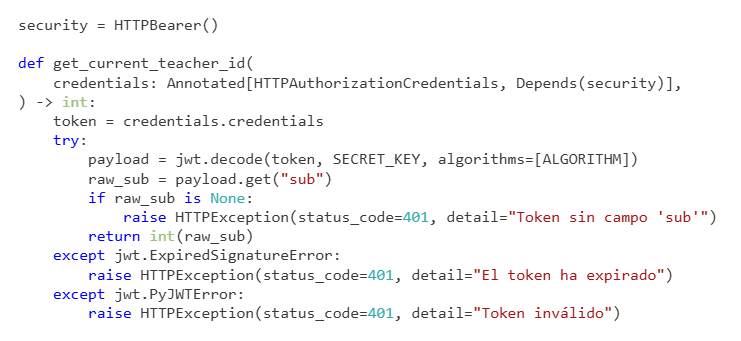
\includegraphics[width=1\textwidth]{listings/autenticacion_jwt_backend.png}}
  \captionof{lstlisting}{Inyección de dependencia para la validación de tokens JWT}
  \label{lst:autenticacion_jwt_backend}
\end{figure}

Esta función intercepta el \textit{Bearer token} emitido en las peticiones HTTP, descifra la firma criptográfica del estándar JSON Web Token~\cite{ietf_jwt_rfc7519} utilizando la clave secreta del servidor (\texttt{SECRET\_KEY}) y verifica su validez temporal antes de permitir el acceso a los controladores protegidos.


\section{Estrategia de testing}\label{sec:estrategia_testing}
Unitarias, integración, E2E, etc

Me gustaría mencionar también su importancia y los objetivos de cobertura que tengo, quizás lo mejor sea en este capítulo mencionar los umbrales objetivos y en el capítulo 9 de resultados hablar de su cumplimiento
\section{Casos de prueba y validación}\label{sec:casos_de_prueba_y_validacion}

Descripción de los casos de prueba utilizados para validar los criterios de aceptación y alcanzar la cobertura objetivo

\section{Pruebas de carga y rendimiento}
Descripción de las pruebas de carga y rendimiento realizadas

Importante porque los cuestionarios son en directo y con muchas personas simultáneamente
